\subsubsection{Addition Operator}

The test takes 10 million positive randomly generated integers and calculates the sum of them. See Figure \ref{fig:native_addition} for results. Other operators such as subtraction, multiplication, division and modulo were also tested but generated the same results.

\begin{figure}[h]
	\centering
	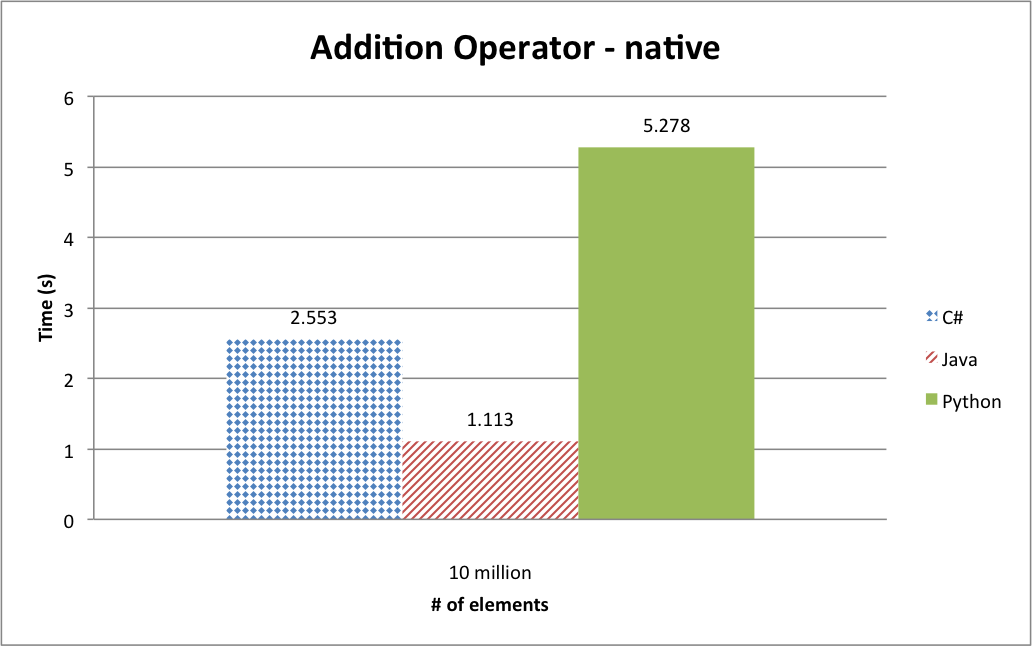
\includegraphics[width=1.0\linewidth]{chapters/new_media/AdditionOperatorNative.png}
	\caption{This tests a language ability to sum 10 million elements. Lower is better. The results show that Java running in its native environment is the fastest of the three languages with 1.113 seconds. Python is the slowest of the three with a runtime of 5.278 seconds, even when using its native library functions to sum the elements, see \ref{appendix:code_addition}.}
	\label{fig:native_addition}
\end{figure}
